%^^^^^^^^^^^^^^^^^^^^^^^^^^^^^^^^^^^^^^^^^^^^^^^^^^^^^^^^^^^^^^^^^^^^^^^^^^^^^^^
%		Immagine della variazione geodetica in un piano 2d
%_______________________________________________________________________________

\documentclass{standalone}

\usepackage{tikz}
%\usetikzlibrary{...}
\usepackage{tikz}
\usepackage{pgfplots}
\pgfplotsset{compat=newest}
\usetikzlibrary{calc}

%Common symbols
%Common math symbols
	%Number fields
		\newcommand{\Real}{\mathbb{R}}
		\newcommand{\Natural}{\mathbb{N}}
		\newcommand{\Relative}{\mathbb{Z}}
		\newcommand{\Rational}{\mathbb{Q}}
		\newcommand{\Complex}{\mathbb{C}}
	
%equality lingo
	%must be equal
		\newcommand{\mbeq}{\overset{!}{=}} 

% function
	%Domain
		\newcommand{\dom}{\mathrm{dom}}
	%Range
		\newcommand{\ran}{\mathrm{ran}}
	

% Set Theory
	% Power set (insieme delle parti
		\newcommand{\PowerSet}{\mathcal{P}}

%Differential Geometry
	% Atlas
		\newcommand{\Atlas}{\mathcal{A}}
	%support
		\newcommand{\supp}{\textrm{supp}}

	
	
%Category Theory
	%Mor set http://ncatlab.org/nlab/show/morphism
%		\newcommand{\hom}{\textrm{hom}}

%Geometric Lagrangian Mechanics
	% Kinematic Configurations
		\newcommand{\Conf}{\mathtt{C}}
	%Solutions Space
		\newcommand{\Sol}{\mathtt{Sol}}
	%Lagrangian class
		\newcommand{\Lag}{\mathsf{Lag}}
	%Lagrangiana
		\newcommand{\Lagrangian}{\mathcal{L}}
	%Data
		\newcommand{\Data}{\mathsf{Data}}
	%unique solution map
		\newcommand{\SolMap}{\mathbf{s}}
	%Classical Observables
		\newcommand{\Obs}{\mathcal{E}}	
	%Phase Space
		\newcommand{\Phase}{\mathcal{M}}	

		\
		
%Peierls (per non sbagliare più)
		\newcommand{\Pei}{Peierls}

\begin{document}
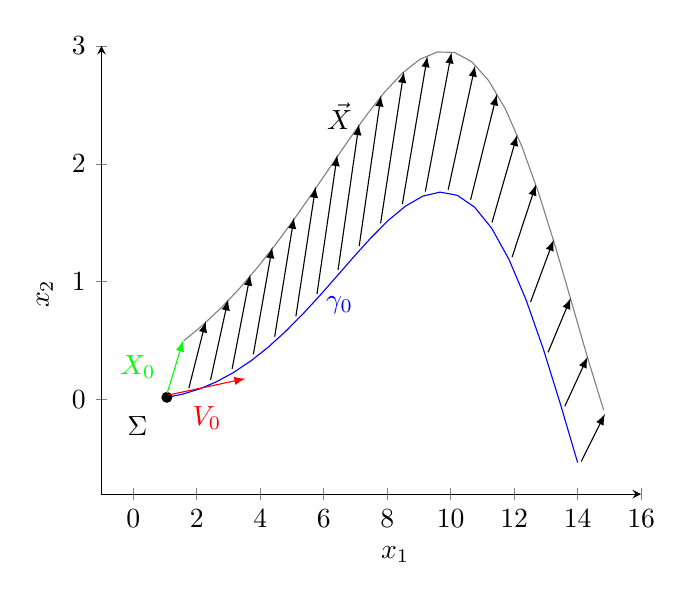
\begin{tikzpicture}
\begin{axis}[	axis x line=bottom, axis y line=left,
						%ticks=none,
						xlabel={$x_1$},ylabel={$x_2$},
						xlabel style={below right},ylabel style={above left},
						xmin=-1, xmax=16, ymin=-0.8, ymax=3
						]
 
 		% Geodesica di partenza
		\addplot[blue,domain=1:14,variable=\t] ({t},{sin(x^2)*x^(1/4)})		
		  \foreach \p in {0,1,...,20}{						%punti per ottenere il vettore variazione
      		node[sloped,inner sep=0cm,above,pos=\p/20,
      			anchor=south west]
      			(N \p){}
  			};	

		% Geodesica Variata
		\addplot[gray,domain=1:14,variable=\t] ({t+0.5*(1+sin(t*10))},{sin(x^2)*x^(1/4)+(1 +0.5*cos(t*10))*t/10+0.3})
			 \foreach \p in {0,1,...,20}{						%punti per ottenere il vettore variazione
    	  		node[	sloped,inner sep=0cm,above,pos=\p/20,
      						anchor=south west]
      				(M \p){}
  			};	

		%I Dati Iniziali
		\fill (N 0.south) circle [radius=2pt]node [label={225:{$\Sigma$}}]  {};  

		\draw[-latex,color=green] (N 0) -- (M 0) node [pos=0.5,label={180:{$X_0$}}]  {};    

		%La velocità iniziale la metto a mano in modo che si legga chiaramente 
		\draw[-latex,color=red] (N 0)  -- ($(N 1) + (0.8,-0.7)$) node [pos=0.5,label={270:{$V_0$}}]  {};
		
		\node[black] at (axis cs:6.5,2.4) {$\vec{X}$};
		\node [blue]  at (axis cs:6.5,0.8)   {$\gamma_0$};

\end{axis}

	%Lo Jacobi Field
    \foreach \p in {1,2,...,20} {
      \draw[-latex,color=black] (N \p) -- (M \p);
    }


\end{tikzpicture}
\end{document}